\documentclass[1p]{elsarticle_modified}
%\bibliographystyle{elsarticle-num}

%\usepackage[colorlinks]{hyperref}
%\usepackage{abbrmath_seonhwa} %\Abb, \Ascr, \Acal ,\Abf, \Afrak
\usepackage{amsfonts}
\usepackage{amssymb}
\usepackage{amsmath}
\usepackage{amsthm}
\usepackage{scalefnt}
\usepackage{amsbsy}
\usepackage{kotex}
\usepackage{caption}
\usepackage{subfig}
\usepackage{color}
\usepackage{graphicx}
\usepackage{xcolor} %% white, black, red, green, blue, cyan, magenta, yellow
\usepackage{float}
\usepackage{setspace}
\usepackage{hyperref}

\usepackage{tikz}
\usetikzlibrary{arrows}

\usepackage{multirow}
\usepackage{array} % fixed length table
\usepackage{hhline}

%%%%%%%%%%%%%%%%%%%%%
\makeatletter
\renewcommand*\env@matrix[1][\arraystretch]{%
	\edef\arraystretch{#1}%
	\hskip -\arraycolsep
	\let\@ifnextchar\new@ifnextchar
	\array{*\c@MaxMatrixCols c}}
\makeatother %https://tex.stackexchange.com/questions/14071/how-can-i-increase-the-line-spacing-in-a-matrix
%%%%%%%%%%%%%%%

\usepackage[normalem]{ulem}

\newcommand{\msout}[1]{\ifmmode\text{\sout{\ensuremath{#1}}}\else\sout{#1}\fi}
%SOURCE: \msout is \stkout macro in https://tex.stackexchange.com/questions/20609/strikeout-in-math-mode

\newcommand{\cancel}[1]{
	\ifmmode
	{\color{red}\msout{#1}}
	\else
	{\color{red}\sout{#1}}
	\fi
}

\newcommand{\add}[1]{
	{\color{blue}\uwave{#1}}
}

\newcommand{\replace}[2]{
	\ifmmode
	{\color{red}\msout{#1}}{\color{blue}\uwave{#2}}
	\else
	{\color{red}\sout{#1}}{\color{blue}\uwave{#2}}
	\fi
}

\newcommand{\Sol}{\mathcal{S}} %segment
\newcommand{\D}{D} %diagram
\newcommand{\A}{\mathcal{A}} %arc


%%%%%%%%%%%%%%%%%%%%%%%%%%%%%5 test

\def\sl{\operatorname{\textup{SL}}(2,\Cbb)}
\def\psl{\operatorname{\textup{PSL}}(2,\Cbb)}
\def\quan{\mkern 1mu \triangleright \mkern 1mu}

\theoremstyle{definition}
\newtheorem{thm}{Theorem}[section]
\newtheorem{prop}[thm]{Proposition}
\newtheorem{lem}[thm]{Lemma}
\newtheorem{ques}[thm]{Question}
\newtheorem{cor}[thm]{Corollary}
\newtheorem{defn}[thm]{Definition}
\newtheorem{exam}[thm]{Example}
\newtheorem{rmk}[thm]{Remark}
\newtheorem{alg}[thm]{Algorithm}

\newcommand{\I}{\sqrt{-1}}
\begin{document}

%\begin{frontmatter}
%
%\title{Boundary parabolic representations of knots up to 8 crossings}
%
%%% Group authors per affiliation:
%\author{Yunhi Cho} 
%\address{Department of Mathematics, University of Seoul, Seoul, Korea}
%\ead{yhcho@uos.ac.kr}
%
%
%\author{Seonhwa Kim} %\fnref{s_kim}}
%\address{Center for Geometry and Physics, Institute for Basic Science, Pohang, 37673, Korea}
%\ead{ryeona17@ibs.re.kr}
%
%\author{Hyuk Kim}
%\address{Department of Mathematical Sciences, Seoul National University, Seoul 08826, Korea}
%\ead{hyukkim@snu.ac.kr}
%
%\author{Seokbeom Yoon}
%\address{Department of Mathematical Sciences, Seoul National University, Seoul, 08826,  Korea}
%\ead{sbyoon15@snu.ac.kr}
%
%\begin{abstract}
%We find all boundary parabolic representation of knots up to 8 crossings.
%
%\end{abstract}
%\begin{keyword}
%    \MSC[2010] 57M25 
%\end{keyword}
%
%\end{frontmatter}

%\linenumbers
%\tableofcontents
%
\newcommand\colored[1]{\textcolor{white}{\rule[-0.35ex]{0.8em}{1.4ex}}\kern-0.8em\color{red} #1}%
%\newcommand\colored[1]{\textcolor{white}{ #1}\kern-2.17ex	\textcolor{white}{ #1}\kern-1.81ex	\textcolor{white}{ #1}\kern-2.15ex\color{red}#1	}

{\Large $\underline{12n_{0224}~(K12n_{0224})}$}

\setlength{\tabcolsep}{10pt}
\renewcommand{\arraystretch}{1.6}
\vspace{1cm}\begin{tabular}{m{100pt}>{\centering\arraybackslash}m{274pt}}
\multirow{5}{120pt}{
	\centering
	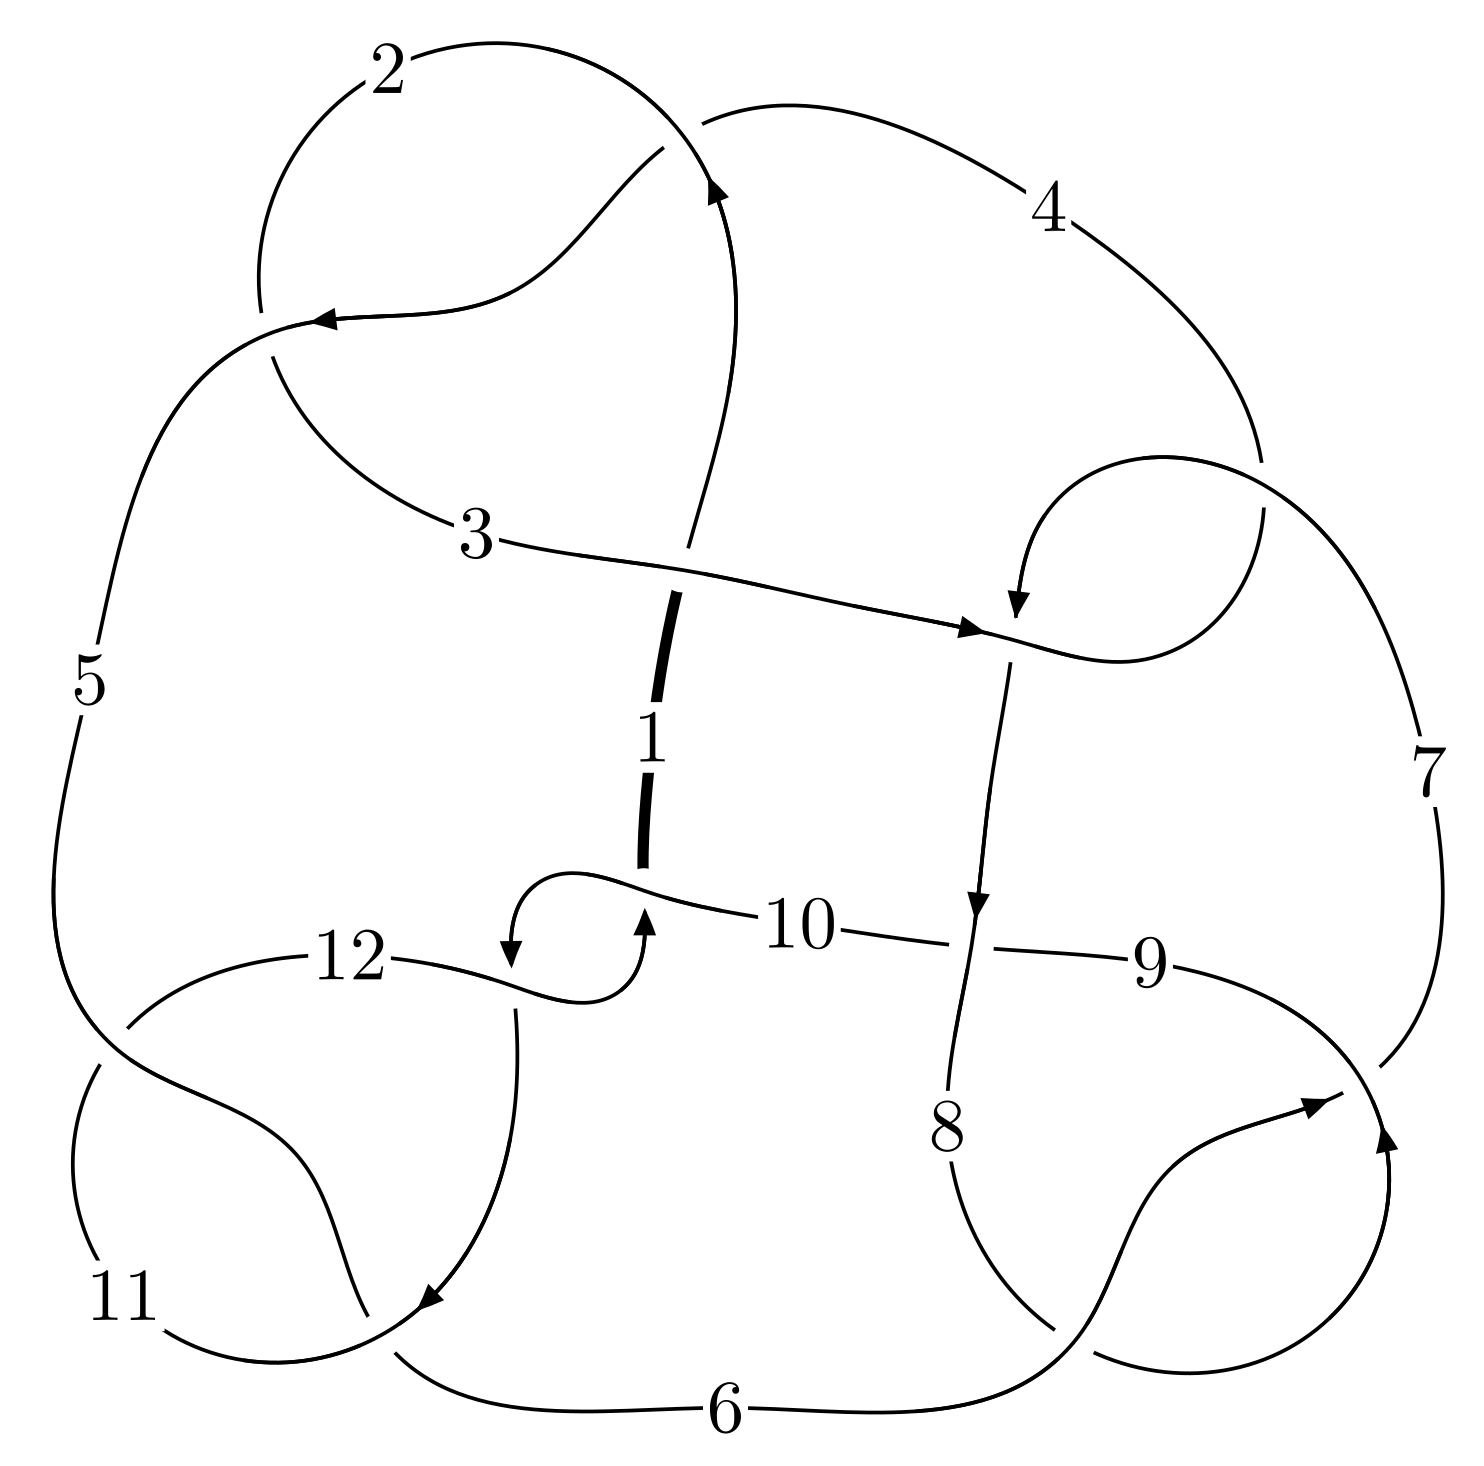
\includegraphics[width=112pt]{../../../GIT/diagram.site/Diagrams/png/2313_12n_0224.png}\\
\ \ \ A knot diagram\footnotemark}&
\allowdisplaybreaks
\textbf{Linearized knot diagam} \\
\cline{2-2}
 &
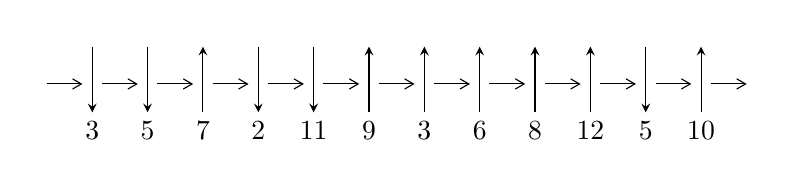
\begin{tikzpicture}[x=20pt, y=17pt]
	% nodes
	\node (C0) at (0, 0) {};
	\node (C1) at (1, 0) {};
	\node (C1U) at (1, +1) {};
	\node (C1D) at (1, -1) {3};

	\node (C2) at (2, 0) {};
	\node (C2U) at (2, +1) {};
	\node (C2D) at (2, -1) {5};

	\node (C3) at (3, 0) {};
	\node (C3U) at (3, +1) {};
	\node (C3D) at (3, -1) {7};

	\node (C4) at (4, 0) {};
	\node (C4U) at (4, +1) {};
	\node (C4D) at (4, -1) {2};

	\node (C5) at (5, 0) {};
	\node (C5U) at (5, +1) {};
	\node (C5D) at (5, -1) {11};

	\node (C6) at (6, 0) {};
	\node (C6U) at (6, +1) {};
	\node (C6D) at (6, -1) {9};

	\node (C7) at (7, 0) {};
	\node (C7U) at (7, +1) {};
	\node (C7D) at (7, -1) {3};

	\node (C8) at (8, 0) {};
	\node (C8U) at (8, +1) {};
	\node (C8D) at (8, -1) {6};

	\node (C9) at (9, 0) {};
	\node (C9U) at (9, +1) {};
	\node (C9D) at (9, -1) {8};

	\node (C10) at (10, 0) {};
	\node (C10U) at (10, +1) {};
	\node (C10D) at (10, -1) {12};

	\node (C11) at (11, 0) {};
	\node (C11U) at (11, +1) {};
	\node (C11D) at (11, -1) {5};

	\node (C12) at (12, 0) {};
	\node (C12U) at (12, +1) {};
	\node (C12D) at (12, -1) {10};
	\node (C13) at (13, 0) {};

	% arrows
	\draw[->,>={angle 60}]
	(C0) edge (C1) (C1) edge (C2) (C2) edge (C3) (C3) edge (C4) (C4) edge (C5) (C5) edge (C6) (C6) edge (C7) (C7) edge (C8) (C8) edge (C9) (C9) edge (C10) (C10) edge (C11) (C11) edge (C12) (C12) edge (C13) ;	\draw[->,>=stealth]
	(C1U) edge (C1D) (C2U) edge (C2D) (C3D) edge (C3U) (C4U) edge (C4D) (C5U) edge (C5D) (C6D) edge (C6U) (C7D) edge (C7U) (C8D) edge (C8U) (C9D) edge (C9U) (C10D) edge (C10U) (C11U) edge (C11D) (C12D) edge (C12U) ;
	\end{tikzpicture} \\
\hhline{~~} \\& 
\textbf{Solving Sequence} \\ \cline{2-2} 
 &
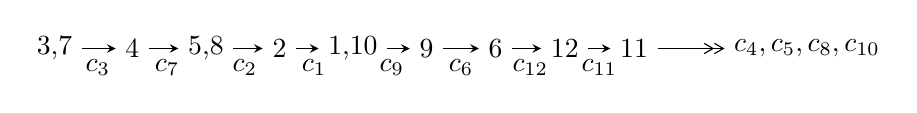
\begin{tikzpicture}[x=25pt, y=7pt]
	% node
	\node (A0) at (-1/8, 0) {3,7};
	\node (A1) at (1, 0) {4};
	\node (A2) at (33/16, 0) {5,8};
	\node (A3) at (25/8, 0) {2};
	\node (A4) at (67/16, 0) {1,10};
	\node (A5) at (21/4, 0) {9};
	\node (A6) at (25/4, 0) {6};
	\node (A7) at (29/4, 0) {12};
	\node (A8) at (33/4, 0) {11};
	\node (C1) at (1/2, -1) {$c_{3}$};
	\node (C2) at (3/2, -1) {$c_{7}$};
	\node (C3) at (21/8, -1) {$c_{2}$};
	\node (C4) at (29/8, -1) {$c_{1}$};
	\node (C5) at (19/4, -1) {$c_{9}$};
	\node (C6) at (23/4, -1) {$c_{6}$};
	\node (C7) at (27/4, -1) {$c_{12}$};
	\node (C8) at (31/4, -1) {$c_{11}$};
	\node (A9) at (43/4, 0) {$c_{4},c_{5},c_{8},c_{10}$};

	% edge
	\draw[->,>=stealth]	
	(A0) edge (A1) (A1) edge (A2) (A2) edge (A3) (A3) edge (A4) (A4) edge (A5) (A5) edge (A6) (A6) edge (A7) (A7) edge (A8) ;
	\draw[->>,>={angle 60}]	
	(A8) edge (A9);
\end{tikzpicture} \\ 

\end{tabular} \\

\footnotetext{
The image of knot diagram is generated by the software ``\textbf{Draw programme}" developed by Andrew Bartholomew(\url{http://www.layer8.co.uk/maths/draw/index.htm\#Running-draw}), where we modified some parts for our purpose(\url{https://github.com/CATsTAILs/LinksPainter}).
}\phantom \\ \newline 
\centering \textbf{Ideals for irreducible components\footnotemark of $X_{\text{par}}$} 
 
\begin{align*}
I^u_{1}&=\langle 
9.65958\times10^{65} u^{40}+1.97140\times10^{66} u^{39}+\cdots+1.18987\times10^{68} d-9.62857\times10^{67},\\
\phantom{I^u_{1}}&\phantom{= \langle  }1.07299\times10^{66} u^{40}+1.97354\times10^{66} u^{39}+\cdots+1.18987\times10^{68} c+6.68255\times10^{67},\\
\phantom{I^u_{1}}&\phantom{= \langle  }-1.37658\times10^{65} u^{40}-4.47424\times10^{65} u^{39}+\cdots+1.06596\times10^{68} b-6.96533\times10^{67},\\
\phantom{I^u_{1}}&\phantom{= \langle  }5.90486\times10^{65} u^{40}+1.83524\times10^{66} u^{39}+\cdots+4.26385\times10^{68} a-3.18493\times10^{67},\\
\phantom{I^u_{1}}&\phantom{= \langle  }u^{41}+2 u^{40}+\cdots-512 u^2-512\rangle \\
I^u_{2}&=\langle 
u^3 a^2+5 u^3 a+2 a^2 u-4 u^2 a-4 u^3+11 a u+4 u^2+d-8 a-10 u+8,\\
\phantom{I^u_{2}}&\phantom{= \langle  }u^3 a^2+3 u^3 a+a^2 u-2 u^2 a-2 u^3+4 a u+2 u^2+c-4 a-4 u+4,\;- a^2 u^2+b+2 a-2,\\
\phantom{I^u_{2}}&\phantom{= \langle  }4 u^3 a^2-2 a^2 u^2-6 u^3 a+a^3+10 a^2 u+3 u^2 a+2 u^3-2 a^2-15 a u- u^2+3 a+5 u-1,\;u^4- u^3+3 u^2-2 u+1\rangle \\
\\
I^v_{1}&=\langle 
c,\;d- v-1,\;b,\;a-1,\;v^2+v+1\rangle \\
I^v_{2}&=\langle 
a,\;d,\;c- v,\;b-1,\;v^2- v+1\rangle \\
I^v_{3}&=\langle 
a,\;d+1,\;c+a,\;b-1,\;v-1\rangle \\
I^v_{4}&=\langle 
a,\;a^2 d- c^2 v-2 c a+c v+a- v,\;d v+1,\;c^2 v^2+2 c a v- v^2 c+a^2- a v+v^2,\;b-1\rangle \\
\end{align*}
\raggedright * 5 irreducible components of $\dim_{\mathbb{C}}=0$, with total 58 representations.\\
\raggedright * 1 irreducible components of $\dim_{\mathbb{C}}=1$ \\
\footnotetext{All coefficients of polynomials are rational numbers. But the coefficients are sometimes approximated in decimal forms when there is not enough margin.}
\newpage
\renewcommand{\arraystretch}{1}
\centering \section*{I. $I^u_{1}= \langle 9.66\times10^{65} u^{40}+1.97\times10^{66} u^{39}+\cdots+1.19\times10^{68} d-9.63\times10^{67},\;1.07\times10^{66} u^{40}+1.97\times10^{66} u^{39}+\cdots+1.19\times10^{68} c+6.68\times10^{67},\;-1.38\times10^{65} u^{40}-4.47\times10^{65} u^{39}+\cdots+1.07\times10^{68} b-6.97\times10^{67},\;5.90\times10^{65} u^{40}+1.84\times10^{66} u^{39}+\cdots+4.26\times10^{68} a-3.18\times10^{67},\;u^{41}+2 u^{40}+\cdots-512 u^2-512 \rangle$}
\flushleft \textbf{(i) Arc colorings}\\
\begin{tabular}{m{7pt} m{180pt} m{7pt} m{180pt} }
\flushright $a_{3}=$&$\begin{pmatrix}1\\0\end{pmatrix}$ \\
\flushright $a_{7}=$&$\begin{pmatrix}0\\u\end{pmatrix}$ \\
\flushright $a_{4}=$&$\begin{pmatrix}1\\- u^2\end{pmatrix}$ \\
\flushright $a_{5}=$&$\begin{pmatrix}-0.00138487 u^{40}-0.00430419 u^{39}+\cdots-1.07263 u+0.0746961\\0.00129140 u^{40}+0.00419737 u^{39}+\cdots+1.25599 u+0.653432\end{pmatrix}$ \\
\flushright $a_{8}=$&$\begin{pmatrix}u\\u\end{pmatrix}$ \\
\flushright $a_{2}=$&$\begin{pmatrix}-0.00138487 u^{40}-0.00430419 u^{39}+\cdots-1.07263 u+0.0746961\\-0.000383620 u^{40}-0.00160154 u^{39}+\cdots-0.546942 u+0.132211\end{pmatrix}$ \\
\flushright $a_{1}=$&$\begin{pmatrix}-0.00176849 u^{40}-0.00590573 u^{39}+\cdots-1.61957 u+0.206907\\-0.000383620 u^{40}-0.00160154 u^{39}+\cdots-0.546942 u+0.132211\end{pmatrix}$ \\
\flushright $a_{10}=$&$\begin{pmatrix}-0.00901765 u^{40}-0.0165861 u^{39}+\cdots+12.4282 u-0.561619\\-0.00811817 u^{40}-0.0165681 u^{39}+\cdots+8.57387 u+0.809210\end{pmatrix}$ \\
\flushright $a_{9}=$&$\begin{pmatrix}-0.00756180 u^{40}-0.0140634 u^{39}+\cdots+11.9677 u+0.350233\\-0.00666231 u^{40}-0.0140454 u^{39}+\cdots+8.11334 u+1.72106\end{pmatrix}$ \\
\flushright $a_{6}=$&$\begin{pmatrix}0.000899485 u^{40}+0.0000180094 u^{39}+\cdots-3.85437 u+1.37083\\-0.00666231 u^{40}-0.0140454 u^{39}+\cdots+8.11334 u+1.72106\end{pmatrix}$ \\
\flushright $a_{12}=$&$\begin{pmatrix}-0.00898279 u^{40}-0.0228872 u^{39}+\cdots+6.35254 u+2.83155\\-0.00602820 u^{40}-0.0101798 u^{39}+\cdots+8.49552 u-2.03570\end{pmatrix}$ \\
\flushright $a_{11}=$&$\begin{pmatrix}-0.00761817 u^{40}-0.0171648 u^{39}+\cdots+9.71421 u+2.83352\\-0.00515696 u^{40}-0.00747593 u^{39}+\cdots+7.91840 u-3.20299\end{pmatrix}$\\&\end{tabular}
\flushleft \textbf{(ii) Obstruction class $= -1$}\\~\\
\flushleft \textbf{(iii) Cusp Shapes $= 0.00750642 u^{40}+0.0137245 u^{39}+\cdots+0.520985 u+10.6626$}\\~\\
\newpage\renewcommand{\arraystretch}{1}
\flushleft \textbf{(iv) u-Polynomials at the component}\newline \\
\begin{tabular}{m{50pt}|m{274pt}}
Crossings & \hspace{64pt}u-Polynomials at each crossing \\
\hline $$\begin{aligned}c_{1}\end{aligned}$$&$\begin{aligned}
&u^{41}+50 u^{40}+\cdots+8224 u+256
\end{aligned}$\\
\hline $$\begin{aligned}c_{2},c_{4}\end{aligned}$$&$\begin{aligned}
&u^{41}-8 u^{40}+\cdots-8 u-16
\end{aligned}$\\
\hline $$\begin{aligned}c_{3},c_{7}\end{aligned}$$&$\begin{aligned}
&u^{41}+2 u^{40}+\cdots-512 u^2-512
\end{aligned}$\\
\hline $$\begin{aligned}c_{5},c_{11}\end{aligned}$$&$\begin{aligned}
&u^{41}-2 u^{40}+\cdots+16 u-4
\end{aligned}$\\
\hline $$\begin{aligned}c_{6},c_{8}\end{aligned}$$&$\begin{aligned}
&u^{41}+8 u^{40}+\cdots-8 u-16
\end{aligned}$\\
\hline $$\begin{aligned}c_{9}\end{aligned}$$&$\begin{aligned}
&u^{41}-10 u^{40}+\cdots+2080 u-256
\end{aligned}$\\
\hline $$\begin{aligned}c_{10},c_{12}\end{aligned}$$&$\begin{aligned}
&u^{41}-12 u^{40}+\cdots+344 u+16
\end{aligned}$\\
\hline
\end{tabular}\\~\\
\newpage\renewcommand{\arraystretch}{1}
\flushleft \textbf{(v) Riley Polynomials at the component}\newline \\
\begin{tabular}{m{50pt}|m{274pt}}
Crossings & \hspace{64pt}Riley Polynomials at each crossing \\
\hline $$\begin{aligned}c_{1}\end{aligned}$$&$\begin{aligned}
&y^{41}-110 y^{40}+\cdots+25092608 y-65536
\end{aligned}$\\
\hline $$\begin{aligned}c_{2},c_{4}\end{aligned}$$&$\begin{aligned}
&y^{41}-50 y^{40}+\cdots+8224 y-256
\end{aligned}$\\
\hline $$\begin{aligned}c_{3},c_{7}\end{aligned}$$&$\begin{aligned}
&y^{41}+30 y^{40}+\cdots-524288 y-262144
\end{aligned}$\\
\hline $$\begin{aligned}c_{5},c_{11}\end{aligned}$$&$\begin{aligned}
&y^{41}+12 y^{40}+\cdots+344 y-16
\end{aligned}$\\
\hline $$\begin{aligned}c_{6},c_{8}\end{aligned}$$&$\begin{aligned}
&y^{41}-10 y^{40}+\cdots+2080 y-256
\end{aligned}$\\
\hline $$\begin{aligned}c_{9}\end{aligned}$$&$\begin{aligned}
&y^{41}+50 y^{40}+\cdots-663040 y-65536
\end{aligned}$\\
\hline $$\begin{aligned}c_{10},c_{12}\end{aligned}$$&$\begin{aligned}
&y^{41}+36 y^{40}+\cdots+135968 y-256
\end{aligned}$\\
\hline
\end{tabular}\\~\\
\newpage\flushleft \textbf{(vi) Complex Volumes and Cusp Shapes}
$$\begin{array}{c|c|c}  
\text{Solutions to }I^u_{1}& \I (\text{vol} + \sqrt{-1}CS) & \text{Cusp shape}\\
 \hline 
\begin{aligned}
u &= -0.280189 + 0.954581 I \\
a &= \phantom{-}0.590964 - 0.259086 I \\
b &= \phantom{-}0.419345 + 0.622257 I \\
c &= \phantom{-}0.0474799 - 0.0430603 I \\
d &= \phantom{-}1.033380 + 0.229578 I\end{aligned}
 & \phantom{-}1.60252 - 4.55290 I & \phantom{-}4.51064 + 8.08001 I \\ \hline\begin{aligned}
u &= -0.280189 - 0.954581 I \\
a &= \phantom{-}0.590964 + 0.259086 I \\
b &= \phantom{-}0.419345 - 0.622257 I \\
c &= \phantom{-}0.0474799 + 0.0430603 I \\
d &= \phantom{-}1.033380 - 0.229578 I\end{aligned}
 & \phantom{-}1.60252 + 4.55290 I & \phantom{-}4.51064 - 8.08001 I \\ \hline\begin{aligned}
u &= -0.942111 + 0.024266 I \\
a &= \phantom{-}0.91333 - 1.27170 I \\
b &= -0.627424 + 0.518765 I \\
c &= -0.499993 + 0.079611 I \\
d &= -0.315261 + 0.806428 I\end{aligned}
 & -0.87865 + 4.07350 I & \phantom{-}1.48942 - 7.36111 I \\ \hline\begin{aligned}
u &= -0.942111 - 0.024266 I \\
a &= \phantom{-}0.91333 + 1.27170 I \\
b &= -0.627424 - 0.518765 I \\
c &= -0.499993 - 0.079611 I \\
d &= -0.315261 - 0.806428 I\end{aligned}
 & -0.87865 - 4.07350 I & \phantom{-}1.48942 + 7.36111 I \\ \hline\begin{aligned}
u &= -0.100000 + 0.892301 I \\
a &= \phantom{-}0.541244 + 0.141055 I \\
b &= \phantom{-}0.730090 - 0.450883 I \\
c &= \phantom{-}0.004841 + 0.674193 I \\
d &= -0.587647 + 0.795464 I\end{aligned}
 & -1.46086 + 1.42227 I & -3.88823 - 3.83998 I \\ \hline\begin{aligned}
u &= -0.100000 - 0.892301 I \\
a &= \phantom{-}0.541244 - 0.141055 I \\
b &= \phantom{-}0.730090 + 0.450883 I \\
c &= \phantom{-}0.004841 - 0.674193 I \\
d &= -0.587647 - 0.795464 I\end{aligned}
 & -1.46086 - 1.42227 I & -3.88823 + 3.83998 I\\
 \hline 
 \end{array}$$\newpage$$\begin{array}{c|c|c}  
\text{Solutions to }I^u_{1}& \I (\text{vol} + \sqrt{-1}CS) & \text{Cusp shape}\\
 \hline 
\begin{aligned}
u &= -0.687957 + 0.421229 I \\
a &= \phantom{-}0.457946 + 0.040164 I \\
b &= \phantom{-}1.167000 - 0.190055 I \\
c &= -0.728909 + 0.390845 I \\
d &= -0.849961 + 0.066792 I\end{aligned}
 & -2.43397 + 0.55461 I & -3.61478 + 1.21885 I \\ \hline\begin{aligned}
u &= -0.687957 - 0.421229 I \\
a &= \phantom{-}0.457946 - 0.040164 I \\
b &= \phantom{-}1.167000 + 0.190055 I \\
c &= -0.728909 - 0.390845 I \\
d &= -0.849961 - 0.066792 I\end{aligned}
 & -2.43397 - 0.55461 I & -3.61478 - 1.21885 I \\ \hline\begin{aligned}
u &= -0.586118 + 0.499909 I \\
a &= \phantom{-}0.841488 - 0.427556 I \\
b &= -0.055470 + 0.479911 I \\
c &= \phantom{-}0.061137 - 1.346250 I \\
d &= \phantom{-}0.633993 + 0.071971 I\end{aligned}
 & \phantom{-}3.14860 + 0.97270 I & \phantom{-}10.27133 - 0.16493 I \\ \hline\begin{aligned}
u &= -0.586118 - 0.499909 I \\
a &= \phantom{-}0.841488 + 0.427556 I \\
b &= -0.055470 - 0.479911 I \\
c &= \phantom{-}0.061137 + 1.346250 I \\
d &= \phantom{-}0.633993 - 0.071971 I\end{aligned}
 & \phantom{-}3.14860 - 0.97270 I & \phantom{-}10.27133 + 0.16493 I \\ \hline\begin{aligned}
u &= \phantom{-}0.757570 + 0.057431 I \\
a &= \phantom{-}1.57773 - 1.54774 I \\
b &= -0.677009 + 0.316853 I \\
c &= \phantom{-}0.629935 + 0.107949 I \\
d &= \phantom{-}0.369651 - 0.357039 I\end{aligned}
 & -0.834104 - 1.057860 I & \phantom{-}1.84303 - 1.72199 I \\ \hline\begin{aligned}
u &= \phantom{-}0.757570 - 0.057431 I \\
a &= \phantom{-}1.57773 + 1.54774 I \\
b &= -0.677009 - 0.316853 I \\
c &= \phantom{-}0.629935 - 0.107949 I \\
d &= \phantom{-}0.369651 + 0.357039 I\end{aligned}
 & -0.834104 + 1.057860 I & \phantom{-}1.84303 + 1.72199 I\\
 \hline 
 \end{array}$$\newpage$$\begin{array}{c|c|c}  
\text{Solutions to }I^u_{1}& \I (\text{vol} + \sqrt{-1}CS) & \text{Cusp shape}\\
 \hline 
\begin{aligned}
u &= \phantom{-}0.748122 + 0.099272 I \\
a &= \phantom{-}0.452596 - 0.009005 I \\
b &= \phantom{-}1.208600 + 0.043942 I \\
c &= \phantom{-}0.532023 - 0.239529 I \\
d &= \phantom{-}0.043520 + 0.421796 I\end{aligned}
 & -0.52179 - 2.81355 I & \phantom{-}3.88749 + 5.15717 I \\ \hline\begin{aligned}
u &= \phantom{-}0.748122 - 0.099272 I \\
a &= \phantom{-}0.452596 + 0.009005 I \\
b &= \phantom{-}1.208600 - 0.043942 I \\
c &= \phantom{-}0.532023 + 0.239529 I \\
d &= \phantom{-}0.043520 - 0.421796 I\end{aligned}
 & -0.52179 + 2.81355 I & \phantom{-}3.88749 - 5.15717 I \\ \hline\begin{aligned}
u &= -0.004283 + 0.652626 I \\
a &= \phantom{-}0.629363 - 0.061738 I \\
b &= \phantom{-}0.573765 + 0.154381 I \\
c &= -0.00038 - 2.68044 I \\
d &= \phantom{-}0.006876 - 0.589549 I\end{aligned}
 & \phantom{-}0.70242 - 2.36927 I & -0.82941 + 4.59716 I \\ \hline\begin{aligned}
u &= -0.004283 - 0.652626 I \\
a &= \phantom{-}0.629363 + 0.061738 I \\
b &= \phantom{-}0.573765 - 0.154381 I \\
c &= -0.00038 + 2.68044 I \\
d &= \phantom{-}0.006876 + 0.589549 I\end{aligned}
 & \phantom{-}0.70242 + 2.36927 I & -0.82941 - 4.59716 I \\ \hline\begin{aligned}
u &= -0.076846 + 0.625583 I \\
a &= \phantom{-}0.695357 - 0.090908 I \\
b &= \phantom{-}0.413943 + 0.184853 I \\
c &= \phantom{-}0.282886 + 0.791726 I \\
d &= \phantom{-}0.74226 + 1.57829 I\end{aligned}
 & \phantom{-}0.85500 + 1.57570 I & \phantom{-}0.179374 + 0.776646 I \\ \hline\begin{aligned}
u &= -0.076846 - 0.625583 I \\
a &= \phantom{-}0.695357 + 0.090908 I \\
b &= \phantom{-}0.413943 - 0.184853 I \\
c &= \phantom{-}0.282886 - 0.791726 I \\
d &= \phantom{-}0.74226 - 1.57829 I\end{aligned}
 & \phantom{-}0.85500 - 1.57570 I & \phantom{-}0.179374 - 0.776646 I\\
 \hline 
 \end{array}$$\newpage$$\begin{array}{c|c|c}  
\text{Solutions to }I^u_{1}& \I (\text{vol} + \sqrt{-1}CS) & \text{Cusp shape}\\
 \hline 
\begin{aligned}
u &= -0.01326 + 1.47518 I \\
a &= -1.81673 + 0.02079 I \\
b &= -1.55037 - 0.00630 I \\
c &= \phantom{-}1.42698 + 0.86838 I \\
d &= \phantom{-}0.490726 + 0.727578 I\end{aligned}
 & -5.83509 - 1.34899 I & -0.977007 + 0.716014 I \\ \hline\begin{aligned}
u &= -0.01326 - 1.47518 I \\
a &= -1.81673 - 0.02079 I \\
b &= -1.55037 + 0.00630 I \\
c &= \phantom{-}1.42698 - 0.86838 I \\
d &= \phantom{-}0.490726 - 0.727578 I\end{aligned}
 & -5.83509 + 1.34899 I & -0.977007 - 0.716014 I \\ \hline\begin{aligned}
u &= \phantom{-}0.45410 + 1.44756 I \\
a &= -1.59641 - 0.64255 I \\
b &= -1.53907 + 0.21697 I \\
c &= \phantom{-}1.49469 - 0.92353 I \\
d &= \phantom{-}0.355963 - 0.961859 I\end{aligned}
 & -4.95290 + 7.65933 I & \phantom{-}2.00000 - 5.62562 I \\ \hline\begin{aligned}
u &= \phantom{-}0.45410 - 1.44756 I \\
a &= -1.59641 + 0.64255 I \\
b &= -1.53907 - 0.21697 I \\
c &= \phantom{-}1.49469 + 0.92353 I \\
d &= \phantom{-}0.355963 + 0.961859 I\end{aligned}
 & -4.95290 - 7.65933 I & \phantom{-}2.00000 + 5.62562 I \\ \hline\begin{aligned}
u &= \phantom{-}0.466919\phantom{ +0.000000I} \\
a &= \phantom{-}1.29906\phantom{ +0.000000I} \\
b &= -0.230214\phantom{ +0.000000I} \\
c &= \phantom{-}1.50297\phantom{ +0.000000I} \\
d &= -0.0988292\phantom{ +0.000000I}\end{aligned}
 & \phantom{-}1.25610\phantom{ +0.000000I} & \phantom{-}8.53770\phantom{ +0.000000I} \\ \hline\begin{aligned}
u &= \phantom{-}0.35061 + 1.53639 I \\
a &= \phantom{-}0.443886 + 0.289097 I \\
b &= \phantom{-}0.581850 - 1.030240 I \\
c &= \phantom{-}1.88732 - 0.49585 I \\
d &= \phantom{-}0.784306 - 0.583648 I\end{aligned}
 & -6.34261 + 3.42138 I & \phantom{-0.000000 } 0\\
 \hline 
 \end{array}$$\newpage$$\begin{array}{c|c|c}  
\text{Solutions to }I^u_{1}& \I (\text{vol} + \sqrt{-1}CS) & \text{Cusp shape}\\
 \hline 
\begin{aligned}
u &= \phantom{-}0.35061 - 1.53639 I \\
a &= \phantom{-}0.443886 - 0.289097 I \\
b &= \phantom{-}0.581850 + 1.030240 I \\
c &= \phantom{-}1.88732 + 0.49585 I \\
d &= \phantom{-}0.784306 + 0.583648 I\end{aligned}
 & -6.34261 - 3.42138 I & \phantom{-0.000000 } 0 \\ \hline\begin{aligned}
u &= -0.51610 + 1.49655 I \\
a &= \phantom{-}0.446462 - 0.321741 I \\
b &= \phantom{-}0.474223 + 1.062390 I \\
c &= -1.68030 - 1.21373 I \\
d &= -0.511523 - 1.269150 I\end{aligned}
 & -5.66064 - 9.73522 I & \phantom{-0.000000 -}0. + 7.05049 I \\ \hline\begin{aligned}
u &= -0.51610 - 1.49655 I \\
a &= \phantom{-}0.446462 + 0.321741 I \\
b &= \phantom{-}0.474223 - 1.062390 I \\
c &= -1.68030 + 1.21373 I \\
d &= -0.511523 + 1.269150 I\end{aligned}
 & -5.66064 + 9.73522 I & \phantom{-0.000000 } 0. - 7.05049 I \\ \hline\begin{aligned}
u &= -1.62020 + 0.13077 I \\
a &= \phantom{-}0.381574 + 0.008996 I \\
b &= \phantom{-}1.61926 - 0.06175 I \\
c &= -0.47751 + 2.12520 I \\
d &= -0.63777 + 3.15512 I\end{aligned}
 & -8.89854 + 0.19005 I & \phantom{-0.000000 } 0 \\ \hline\begin{aligned}
u &= -1.62020 - 0.13077 I \\
a &= \phantom{-}0.381574 - 0.008996 I \\
b &= \phantom{-}1.61926 + 0.06175 I \\
c &= -0.47751 - 2.12520 I \\
d &= -0.63777 - 3.15512 I\end{aligned}
 & -8.89854 - 0.19005 I & \phantom{-0.000000 } 0 \\ \hline\begin{aligned}
u &= \phantom{-}1.59450 + 0.33027 I \\
a &= \phantom{-}0.382027 - 0.022906 I \\
b &= \phantom{-}1.60824 + 0.15639 I \\
c &= -0.39612 + 2.13768 I \\
d &= -0.28184 + 3.24036 I\end{aligned}
 & -8.54414 - 6.61454 I & \phantom{-0.000000 } 0\\
 \hline 
 \end{array}$$\newpage$$\begin{array}{c|c|c}  
\text{Solutions to }I^u_{1}& \I (\text{vol} + \sqrt{-1}CS) & \text{Cusp shape}\\
 \hline 
\begin{aligned}
u &= \phantom{-}1.59450 - 0.33027 I \\
a &= \phantom{-}0.382027 + 0.022906 I \\
b &= \phantom{-}1.60824 - 0.15639 I \\
c &= -0.39612 - 2.13768 I \\
d &= -0.28184 - 3.24036 I\end{aligned}
 & -8.54414 + 6.61454 I & \phantom{-0.000000 } 0 \\ \hline\begin{aligned}
u &= -0.23388 + 1.65276 I \\
a &= -1.52839 + 0.26544 I \\
b &= -1.63512 - 0.11031 I \\
c &= -2.35058 + 0.06091 I \\
d &= -1.275640 - 0.091209 I\end{aligned}
 & -9.70458 - 3.47853 I & \phantom{-0.000000 } 0 \\ \hline\begin{aligned}
u &= -0.23388 - 1.65276 I \\
a &= -1.52839 - 0.26544 I \\
b &= -1.63512 + 0.11031 I \\
c &= -2.35058 - 0.06091 I \\
d &= -1.275640 + 0.091209 I\end{aligned}
 & -9.70458 + 3.47853 I & \phantom{-0.000000 } 0 \\ \hline\begin{aligned}
u &= \phantom{-}0.86658 + 1.51028 I \\
a &= -1.140130 - 0.820998 I \\
b &= -1.57759 + 0.41592 I \\
c &= \phantom{-}1.38502 - 2.89598 I \\
d &= \phantom{-}0.08526 - 2.95483 I\end{aligned}
 & -12.2320 + 15.1490 I & \phantom{-0.000000 } 0 \\ \hline\begin{aligned}
u &= \phantom{-}0.86658 - 1.51028 I \\
a &= -1.140130 + 0.820998 I \\
b &= -1.57759 - 0.41592 I \\
c &= \phantom{-}1.38502 + 2.89598 I \\
d &= \phantom{-}0.08526 + 2.95483 I\end{aligned}
 & -12.2320 - 15.1490 I & \phantom{-0.000000 } 0 \\ \hline\begin{aligned}
u &= -0.78943 + 1.61251 I \\
a &= -1.175700 + 0.706741 I \\
b &= -1.62479 - 0.37558 I \\
c &= -2.01798 - 2.64036 I \\
d &= -0.74497 - 2.73152 I\end{aligned}
 & -13.5026 - 8.6555 I & \phantom{-0.000000 } 0\\
 \hline 
 \end{array}$$\newpage$$\begin{array}{c|c|c}  
\text{Solutions to }I^u_{1}& \I (\text{vol} + \sqrt{-1}CS) & \text{Cusp shape}\\
 \hline 
\begin{aligned}
u &= -0.78943 - 1.61251 I \\
a &= -1.175700 - 0.706741 I \\
b &= -1.62479 + 0.37558 I \\
c &= -2.01798 + 2.64036 I \\
d &= -0.74497 + 2.73152 I\end{aligned}
 & -13.5026 + 8.6555 I & \phantom{-0.000000 } 0 \\ \hline\begin{aligned}
u &= -0.64330 + 1.72758 I \\
a &= -1.231740 + 0.552038 I \\
b &= -1.67606 - 0.30300 I \\
c &= \phantom{-}0.70493 + 3.45324 I \\
d &= -0.14309 + 3.02959 I\end{aligned}
 & -14.7932 - 7.9945 I & \phantom{-0.000000 } 0 \\ \hline\begin{aligned}
u &= -0.64330 - 1.72758 I \\
a &= -1.231740 - 0.552038 I \\
b &= -1.67606 + 0.30300 I \\
c &= \phantom{-}0.70493 - 3.45324 I \\
d &= -0.14309 - 3.02959 I\end{aligned}
 & -14.7932 + 7.9945 I & \phantom{-0.000000 } 0 \\ \hline\begin{aligned}
u &= \phantom{-}0.48873 + 1.82349 I \\
a &= -1.264400 - 0.401956 I \\
b &= -1.71830 + 0.22835 I \\
c &= -1.55696 + 3.30101 I \\
d &= -0.64880 + 2.90927 I\end{aligned}
 & -15.6167 + 1.2657 I & \phantom{-0.000000 } 0 \\ \hline\begin{aligned}
u &= \phantom{-}0.48873 - 1.82349 I \\
a &= -1.264400 + 0.401956 I \\
b &= -1.71830 - 0.22835 I \\
c &= -1.55696 - 3.30101 I \\
d &= -0.64880 - 2.90927 I\end{aligned}
 & -15.6167 - 1.2657 I & \phantom{-0.000000 } 0\\
 \hline 
 \end{array}$$\newpage\newpage\renewcommand{\arraystretch}{1}
\centering \section*{II. $I^u_{2}= \langle u^3 a^2+5 u^3 a+\cdots-8 a+8,\;u^3 a^2+3 u^3 a+\cdots-4 a+4,\;- a^2 u^2+b+2 a-2,\;4 u^3 a^2-6 u^3 a+\cdots+3 a-1,\;u^4- u^3+3 u^2-2 u+1 \rangle$}
\flushleft \textbf{(i) Arc colorings}\\
\begin{tabular}{m{7pt} m{180pt} m{7pt} m{180pt} }
\flushright $a_{3}=$&$\begin{pmatrix}1\\0\end{pmatrix}$ \\
\flushright $a_{7}=$&$\begin{pmatrix}0\\u\end{pmatrix}$ \\
\flushright $a_{4}=$&$\begin{pmatrix}1\\- u^2\end{pmatrix}$ \\
\flushright $a_{5}=$&$\begin{pmatrix}a\\a^2 u^2-2 a+2\end{pmatrix}$ \\
\flushright $a_{8}=$&$\begin{pmatrix}u\\u\end{pmatrix}$ \\
\flushright $a_{2}=$&$\begin{pmatrix}a\\- a^2 u^2- u^2 a+2 a-2\end{pmatrix}$ \\
\flushright $a_{1}=$&$\begin{pmatrix}- a^2 u^2- u^2 a+3 a-2\\- a^2 u^2- u^2 a+2 a-2\end{pmatrix}$ \\
\flushright $a_{10}=$&$\begin{pmatrix}- u^3 a^2-3 u^3 a- a^2 u+2 u^2 a+2 u^3-4 a u-2 u^2+4 a+4 u-4\\- u^3 a^2-5 u^3 a-2 a^2 u+4 u^2 a+4 u^3-11 a u-4 u^2+8 a+10 u-8\end{pmatrix}$ \\
\flushright $a_{9}=$&$\begin{pmatrix}-2 u^3 a- a^2 u+2 u^2 a+2 u^3-6 a u-2 u^2+4 a+6 u-4\\-4 u^3 a-2 a^2 u+4 u^2 a+4 u^3-13 a u-4 u^2+8 a+12 u-8\end{pmatrix}$ \\
\flushright $a_{6}=$&$\begin{pmatrix}-2 u^3 a- a^2 u+2 u^2 a+2 u^3-7 a u-2 u^2+4 a+6 u-4\\-4 u^3 a-2 a^2 u+4 u^2 a+4 u^3-13 a u-4 u^2+8 a+12 u-8\end{pmatrix}$ \\
\flushright $a_{12}=$&$\begin{pmatrix}- u^3 a^2+a^2 u^2- u^3 a-2 a^2 u+4 u^2 a+a^2-2 a u-2 u^2+6 a-4\\- u^3 a^2- u^3 a-2 a^2 u+3 u^2 a+a^2-2 a u-2 u^2+7 a-6\end{pmatrix}$ \\
\flushright $a_{11}=$&$\begin{pmatrix}- u^3 a^2+a^2 u^2-2 a^2 u+3 u^2 a+a^2-2 u^2+5 a-4\\-2 u^3 a^2-3 u^3 a+\cdots+9 a-8\end{pmatrix}$\\&\end{tabular}
\flushleft \textbf{(ii) Obstruction class $= -1$}\\~\\
\flushleft \textbf{(iii) Cusp Shapes $= -4 u^3+4 u^2-12 u+6$}\\~\\
\newpage\renewcommand{\arraystretch}{1}
\flushleft \textbf{(iv) u-Polynomials at the component}\newline \\
\begin{tabular}{m{50pt}|m{274pt}}
Crossings & \hspace{64pt}u-Polynomials at each crossing \\
\hline $$\begin{aligned}c_{1}\end{aligned}$$&$\begin{aligned}
&u^{12}+8 u^{11}+\cdots-10 u+1
\end{aligned}$\\
\hline $$\begin{aligned}c_{2},c_{4},c_{6}\\c_{8}\end{aligned}$$&$\begin{aligned}
&u^{12}-4 u^{10}+\cdots+2 u+1
\end{aligned}$\\
\hline $$\begin{aligned}c_{3},c_{7},c_{10}\\c_{12}\end{aligned}$$&$\begin{aligned}
&(u^4- u^3+3 u^2-2 u+1)^3
\end{aligned}$\\
\hline $$\begin{aligned}c_{5},c_{11}\end{aligned}$$&$\begin{aligned}
&(u^4- u^3+u^2+1)^3
\end{aligned}$\\
\hline $$\begin{aligned}c_{9}\end{aligned}$$&$\begin{aligned}
&u^{12}-8 u^{11}+\cdots+10 u+1
\end{aligned}$\\
\hline
\end{tabular}\\~\\
\newpage\renewcommand{\arraystretch}{1}
\flushleft \textbf{(v) Riley Polynomials at the component}\newline \\
\begin{tabular}{m{50pt}|m{274pt}}
Crossings & \hspace{64pt}Riley Polynomials at each crossing \\
\hline $$\begin{aligned}c_{1},c_{9}\end{aligned}$$&$\begin{aligned}
&y^{12}-8 y^{11}+\cdots-78 y+1
\end{aligned}$\\
\hline $$\begin{aligned}c_{2},c_{4},c_{6}\\c_{8}\end{aligned}$$&$\begin{aligned}
&y^{12}-8 y^{11}+\cdots+10 y+1
\end{aligned}$\\
\hline $$\begin{aligned}c_{3},c_{7},c_{10}\\c_{12}\end{aligned}$$&$\begin{aligned}
&(y^4+5 y^3+7 y^2+2 y+1)^3
\end{aligned}$\\
\hline $$\begin{aligned}c_{5},c_{11}\end{aligned}$$&$\begin{aligned}
&(y^4+y^3+3 y^2+2 y+1)^3
\end{aligned}$\\
\hline
\end{tabular}\\~\\
\newpage\flushleft \textbf{(vi) Complex Volumes and Cusp Shapes}
$$\begin{array}{c|c|c}  
\text{Solutions to }I^u_{2}& \I (\text{vol} + \sqrt{-1}CS) & \text{Cusp shape}\\
 \hline 
\begin{aligned}
u &= \phantom{-}0.395123 + 0.506844 I \\
a &= \phantom{-}0.837889 + 0.280931 I \\
b &= \phantom{-}0.072869 - 0.359716 I \\
c &= \phantom{-}0.394185 + 0.517164 I \\
d &= \phantom{-}0.577230 + 0.415041 I\end{aligned}
 & \phantom{-}0.21101 + 1.41510 I & \phantom{-}1.82674 - 4.90874 I \\ \hline\begin{aligned}
u &= \phantom{-}0.395123 + 0.506844 I \\
a &= \phantom{-}0.492884 - 0.048733 I \\
b &= \phantom{-}1.009230 + 0.198659 I \\
c &= -1.39293 + 0.39378 I \\
d &= -2.82169 + 1.21168 I\end{aligned}
 & \phantom{-}0.21101 + 1.41510 I & \phantom{-}1.82674 - 4.90874 I \\ \hline\begin{aligned}
u &= \phantom{-}0.395123 + 0.506844 I \\
a &= -2.51225 - 4.92832 I \\
b &= -1.082100 + 0.161058 I \\
c &= \phantom{-}0.20850 - 1.92463 I \\
d &= -0.459158 - 0.186039 I\end{aligned}
 & \phantom{-}0.21101 + 1.41510 I & \phantom{-}1.82674 - 4.90874 I \\ \hline\begin{aligned}
u &= \phantom{-}0.395123 - 0.506844 I \\
a &= \phantom{-}0.837889 - 0.280931 I \\
b &= \phantom{-}0.072869 + 0.359716 I \\
c &= \phantom{-}0.394185 - 0.517164 I \\
d &= \phantom{-}0.577230 - 0.415041 I\end{aligned}
 & \phantom{-}0.21101 - 1.41510 I & \phantom{-}1.82674 + 4.90874 I \\ \hline\begin{aligned}
u &= \phantom{-}0.395123 - 0.506844 I \\
a &= \phantom{-}0.492884 + 0.048733 I \\
b &= \phantom{-}1.009230 - 0.198659 I \\
c &= -1.39293 - 0.39378 I \\
d &= -2.82169 - 1.21168 I\end{aligned}
 & \phantom{-}0.21101 - 1.41510 I & \phantom{-}1.82674 + 4.90874 I \\ \hline\begin{aligned}
u &= \phantom{-}0.395123 - 0.506844 I \\
a &= -2.51225 + 4.92832 I \\
b &= -1.082100 - 0.161058 I \\
c &= \phantom{-}0.20850 + 1.92463 I \\
d &= -0.459158 + 0.186039 I\end{aligned}
 & \phantom{-}0.21101 - 1.41510 I & \phantom{-}1.82674 + 4.90874 I\\
 \hline 
 \end{array}$$\newpage$$\begin{array}{c|c|c}  
\text{Solutions to }I^u_{2}& \I (\text{vol} + \sqrt{-1}CS) & \text{Cusp shape}\\
 \hline 
\begin{aligned}
u &= \phantom{-}0.10488 + 1.55249 I \\
a &= \phantom{-}0.439878 + 0.246240 I \\
b &= \phantom{-}0.730940 - 0.968963 I \\
c &= -1.56704 + 1.28737 I \\
d &= -0.641253 + 1.089290 I\end{aligned}
 & -6.79074 + 3.16396 I & -1.82674 - 2.56480 I \\ \hline\begin{aligned}
u &= \phantom{-}0.10488 + 1.55249 I \\
a &= \phantom{-}0.432622 - 0.214254 I \\
b &= \phantom{-}0.856215 + 0.919282 I \\
c &= \phantom{-}1.82916 + 0.51793 I \\
d &= \phantom{-}0.824626 + 0.377943 I\end{aligned}
 & -6.79074 + 3.16396 I & -1.82674 - 2.56480 I \\ \hline\begin{aligned}
u &= \phantom{-}0.10488 + 1.55249 I \\
a &= -1.69102 - 0.14308 I \\
b &= -1.58715 + 0.04968 I \\
c &= -0.47187 - 4.91028 I \\
d &= -0.47976 - 3.28982 I\end{aligned}
 & -6.79074 + 3.16396 I & -1.82674 - 2.56480 I \\ \hline\begin{aligned}
u &= \phantom{-}0.10488 - 1.55249 I \\
a &= \phantom{-}0.439878 - 0.246240 I \\
b &= \phantom{-}0.730940 + 0.968963 I \\
c &= -1.56704 - 1.28737 I \\
d &= -0.641253 - 1.089290 I\end{aligned}
 & -6.79074 - 3.16396 I & -1.82674 + 2.56480 I \\ \hline\begin{aligned}
u &= \phantom{-}0.10488 - 1.55249 I \\
a &= \phantom{-}0.432622 + 0.214254 I \\
b &= \phantom{-}0.856215 - 0.919282 I \\
c &= \phantom{-}1.82916 - 0.51793 I \\
d &= \phantom{-}0.824626 - 0.377943 I\end{aligned}
 & -6.79074 - 3.16396 I & -1.82674 + 2.56480 I \\ \hline\begin{aligned}
u &= \phantom{-}0.10488 - 1.55249 I \\
a &= -1.69102 + 0.14308 I \\
b &= -1.58715 - 0.04968 I \\
c &= -0.47187 + 4.91028 I \\
d &= -0.47976 + 3.28982 I\end{aligned}
 & -6.79074 - 3.16396 I & -1.82674 + 2.56480 I\\
 \hline 
 \end{array}$$\newpage\newpage\renewcommand{\arraystretch}{1}
\centering \section*{III. $I^v_{1}= \langle c,\;d- v-1,\;b,\;a-1,\;v^2+v+1 \rangle$}
\flushleft \textbf{(i) Arc colorings}\\
\begin{tabular}{m{7pt} m{180pt} m{7pt} m{180pt} }
\flushright $a_{3}=$&$\begin{pmatrix}1\\0\end{pmatrix}$ \\
\flushright $a_{7}=$&$\begin{pmatrix}v\\0\end{pmatrix}$ \\
\flushright $a_{4}=$&$\begin{pmatrix}1\\0\end{pmatrix}$ \\
\flushright $a_{5}=$&$\begin{pmatrix}1\\0\end{pmatrix}$ \\
\flushright $a_{8}=$&$\begin{pmatrix}v\\0\end{pmatrix}$ \\
\flushright $a_{2}=$&$\begin{pmatrix}1\\0\end{pmatrix}$ \\
\flushright $a_{1}=$&$\begin{pmatrix}1\\0\end{pmatrix}$ \\
\flushright $a_{10}=$&$\begin{pmatrix}0\\v+1\end{pmatrix}$ \\
\flushright $a_{9}=$&$\begin{pmatrix}v\\v+1\end{pmatrix}$ \\
\flushright $a_{6}=$&$\begin{pmatrix}0\\- v-1\end{pmatrix}$ \\
\flushright $a_{12}=$&$\begin{pmatrix}1\\v\end{pmatrix}$ \\
\flushright $a_{11}=$&$\begin{pmatrix}v+1\\v\end{pmatrix}$\\&\end{tabular}
\flushleft \textbf{(ii) Obstruction class $= 1$}\\~\\
\flushleft \textbf{(iii) Cusp Shapes $= -4 v+7$}\\~\\
\newpage\renewcommand{\arraystretch}{1}
\flushleft \textbf{(iv) u-Polynomials at the component}\newline \\
\begin{tabular}{m{50pt}|m{274pt}}
Crossings & \hspace{64pt}u-Polynomials at each crossing \\
\hline $$\begin{aligned}c_{1},c_{2},c_{3}\\c_{4},c_{7}\end{aligned}$$&$\begin{aligned}
&u^2
\end{aligned}$\\
\hline $$\begin{aligned}c_{5},c_{10}\end{aligned}$$&$\begin{aligned}
&u^2+u+1
\end{aligned}$\\
\hline $$\begin{aligned}c_{6}\end{aligned}$$&$\begin{aligned}
&(u+1)^2
\end{aligned}$\\
\hline $$\begin{aligned}c_{8},c_{9}\end{aligned}$$&$\begin{aligned}
&(u-1)^2
\end{aligned}$\\
\hline $$\begin{aligned}c_{11},c_{12}\end{aligned}$$&$\begin{aligned}
&u^2- u+1
\end{aligned}$\\
\hline
\end{tabular}\\~\\
\newpage\renewcommand{\arraystretch}{1}
\flushleft \textbf{(v) Riley Polynomials at the component}\newline \\
\begin{tabular}{m{50pt}|m{274pt}}
Crossings & \hspace{64pt}Riley Polynomials at each crossing \\
\hline $$\begin{aligned}c_{1},c_{2},c_{3}\\c_{4},c_{7}\end{aligned}$$&$\begin{aligned}
&y^2
\end{aligned}$\\
\hline $$\begin{aligned}c_{5},c_{10},c_{11}\\c_{12}\end{aligned}$$&$\begin{aligned}
&y^2+y+1
\end{aligned}$\\
\hline $$\begin{aligned}c_{6},c_{8},c_{9}\end{aligned}$$&$\begin{aligned}
&(y-1)^2
\end{aligned}$\\
\hline
\end{tabular}\\~\\
\newpage\flushleft \textbf{(vi) Complex Volumes and Cusp Shapes}
$$\begin{array}{c|c|c}  
\text{Solutions to }I^v_{1}& \I (\text{vol} + \sqrt{-1}CS) & \text{Cusp shape}\\
 \hline 
\begin{aligned}
v &= -0.500000 + 0.866025 I \\
a &= \phantom{-}1.00000\phantom{ +0.000000I} \\
b &= \phantom{-0.000000 } 0 \\
c &= \phantom{-0.000000 } 0 \\
d &= \phantom{-}0.500000 + 0.866025 I\end{aligned}
 & \phantom{-}1.64493 + 2.02988 I & \phantom{-}9.00000 - 3.46410 I \\ \hline\begin{aligned}
v &= -0.500000 - 0.866025 I \\
a &= \phantom{-}1.00000\phantom{ +0.000000I} \\
b &= \phantom{-0.000000 } 0 \\
c &= \phantom{-0.000000 } 0 \\
d &= \phantom{-}0.500000 - 0.866025 I\end{aligned}
 & \phantom{-}1.64493 - 2.02988 I & \phantom{-}9.00000 + 3.46410 I\\
 \hline 
 \end{array}$$\newpage\newpage\renewcommand{\arraystretch}{1}
\centering \section*{IV. $I^v_{2}= \langle a,\;d,\;c- v,\;b-1,\;v^2- v+1 \rangle$}
\flushleft \textbf{(i) Arc colorings}\\
\begin{tabular}{m{7pt} m{180pt} m{7pt} m{180pt} }
\flushright $a_{3}=$&$\begin{pmatrix}1\\0\end{pmatrix}$ \\
\flushright $a_{7}=$&$\begin{pmatrix}v\\0\end{pmatrix}$ \\
\flushright $a_{4}=$&$\begin{pmatrix}1\\0\end{pmatrix}$ \\
\flushright $a_{5}=$&$\begin{pmatrix}0\\1\end{pmatrix}$ \\
\flushright $a_{8}=$&$\begin{pmatrix}v\\0\end{pmatrix}$ \\
\flushright $a_{2}=$&$\begin{pmatrix}1\\-1\end{pmatrix}$ \\
\flushright $a_{1}=$&$\begin{pmatrix}0\\-1\end{pmatrix}$ \\
\flushright $a_{10}=$&$\begin{pmatrix}v\\0\end{pmatrix}$ \\
\flushright $a_{9}=$&$\begin{pmatrix}v\\0\end{pmatrix}$ \\
\flushright $a_{6}=$&$\begin{pmatrix}v\\0\end{pmatrix}$ \\
\flushright $a_{12}=$&$\begin{pmatrix}v-1\\-1\end{pmatrix}$ \\
\flushright $a_{11}=$&$\begin{pmatrix}v-1\\- v\end{pmatrix}$\\&\end{tabular}
\flushleft \textbf{(ii) Obstruction class $= 1$}\\~\\
\flushleft \textbf{(iii) Cusp Shapes $= -4 v-1$}\\~\\
\newpage\renewcommand{\arraystretch}{1}
\flushleft \textbf{(iv) u-Polynomials at the component}\newline \\
\begin{tabular}{m{50pt}|m{274pt}}
Crossings & \hspace{64pt}u-Polynomials at each crossing \\
\hline $$\begin{aligned}c_{1},c_{2}\end{aligned}$$&$\begin{aligned}
&(u-1)^2
\end{aligned}$\\
\hline $$\begin{aligned}c_{3},c_{6},c_{7}\\c_{8},c_{9}\end{aligned}$$&$\begin{aligned}
&u^2
\end{aligned}$\\
\hline $$\begin{aligned}c_{4}\end{aligned}$$&$\begin{aligned}
&(u+1)^2
\end{aligned}$\\
\hline $$\begin{aligned}c_{5},c_{12}\end{aligned}$$&$\begin{aligned}
&u^2- u+1
\end{aligned}$\\
\hline $$\begin{aligned}c_{10},c_{11}\end{aligned}$$&$\begin{aligned}
&u^2+u+1
\end{aligned}$\\
\hline
\end{tabular}\\~\\
\newpage\renewcommand{\arraystretch}{1}
\flushleft \textbf{(v) Riley Polynomials at the component}\newline \\
\begin{tabular}{m{50pt}|m{274pt}}
Crossings & \hspace{64pt}Riley Polynomials at each crossing \\
\hline $$\begin{aligned}c_{1},c_{2},c_{4}\end{aligned}$$&$\begin{aligned}
&(y-1)^2
\end{aligned}$\\
\hline $$\begin{aligned}c_{3},c_{6},c_{7}\\c_{8},c_{9}\end{aligned}$$&$\begin{aligned}
&y^2
\end{aligned}$\\
\hline $$\begin{aligned}c_{5},c_{10},c_{11}\\c_{12}\end{aligned}$$&$\begin{aligned}
&y^2+y+1
\end{aligned}$\\
\hline
\end{tabular}\\~\\
\newpage\flushleft \textbf{(vi) Complex Volumes and Cusp Shapes}
$$\begin{array}{c|c|c}  
\text{Solutions to }I^v_{2}& \I (\text{vol} + \sqrt{-1}CS) & \text{Cusp shape}\\
 \hline 
\begin{aligned}
v &= \phantom{-}0.500000 + 0.866025 I \\
a &= \phantom{-0.000000 } 0 \\
b &= \phantom{-}1.00000\phantom{ +0.000000I} \\
c &= \phantom{-}0.500000 + 0.866025 I \\
d &= \phantom{-0.000000 } 0\end{aligned}
 & -1.64493 + 2.02988 I & -3.00000 - 3.46410 I \\ \hline\begin{aligned}
v &= \phantom{-}0.500000 - 0.866025 I \\
a &= \phantom{-0.000000 } 0 \\
b &= \phantom{-}1.00000\phantom{ +0.000000I} \\
c &= \phantom{-}0.500000 - 0.866025 I \\
d &= \phantom{-0.000000 } 0\end{aligned}
 & -1.64493 - 2.02988 I & -3.00000 + 3.46410 I\\
 \hline 
 \end{array}$$\newpage\newpage\renewcommand{\arraystretch}{1}
\centering \section*{V. $I^v_{3}= \langle a,\;d+1,\;c+a,\;b-1,\;v-1 \rangle$}
\flushleft \textbf{(i) Arc colorings}\\
\begin{tabular}{m{7pt} m{180pt} m{7pt} m{180pt} }
\flushright $a_{3}=$&$\begin{pmatrix}1\\0\end{pmatrix}$ \\
\flushright $a_{7}=$&$\begin{pmatrix}1\\0\end{pmatrix}$ \\
\flushright $a_{4}=$&$\begin{pmatrix}1\\0\end{pmatrix}$ \\
\flushright $a_{5}=$&$\begin{pmatrix}0\\1\end{pmatrix}$ \\
\flushright $a_{8}=$&$\begin{pmatrix}1\\0\end{pmatrix}$ \\
\flushright $a_{2}=$&$\begin{pmatrix}1\\-1\end{pmatrix}$ \\
\flushright $a_{1}=$&$\begin{pmatrix}0\\-1\end{pmatrix}$ \\
\flushright $a_{10}=$&$\begin{pmatrix}0\\-1\end{pmatrix}$ \\
\flushright $a_{9}=$&$\begin{pmatrix}1\\-1\end{pmatrix}$ \\
\flushright $a_{6}=$&$\begin{pmatrix}0\\1\end{pmatrix}$ \\
\flushright $a_{12}=$&$\begin{pmatrix}0\\-1\end{pmatrix}$ \\
\flushright $a_{11}=$&$\begin{pmatrix}0\\-1\end{pmatrix}$\\&\end{tabular}
\flushleft \textbf{(ii) Obstruction class $= 1$}\\~\\
\flushleft \textbf{(iii) Cusp Shapes $= 0$}\\~\\
\newpage\renewcommand{\arraystretch}{1}
\flushleft \textbf{(iv) u-Polynomials at the component}\newline \\
\begin{tabular}{m{50pt}|m{274pt}}
Crossings & \hspace{64pt}u-Polynomials at each crossing \\
\hline $$\begin{aligned}c_{1},c_{2},c_{8}\\c_{9}\end{aligned}$$&$\begin{aligned}
&u-1
\end{aligned}$\\
\hline $$\begin{aligned}c_{3},c_{5},c_{7}\\c_{10},c_{11},c_{12}\end{aligned}$$&$\begin{aligned}
&u
\end{aligned}$\\
\hline $$\begin{aligned}c_{4},c_{6}\end{aligned}$$&$\begin{aligned}
&u+1
\end{aligned}$\\
\hline
\end{tabular}\\~\\
\newpage\renewcommand{\arraystretch}{1}
\flushleft \textbf{(v) Riley Polynomials at the component}\newline \\
\begin{tabular}{m{50pt}|m{274pt}}
Crossings & \hspace{64pt}Riley Polynomials at each crossing \\
\hline $$\begin{aligned}c_{1},c_{2},c_{4}\\c_{6},c_{8},c_{9}\end{aligned}$$&$\begin{aligned}
&y-1
\end{aligned}$\\
\hline $$\begin{aligned}c_{3},c_{5},c_{7}\\c_{10},c_{11},c_{12}\end{aligned}$$&$\begin{aligned}
&y
\end{aligned}$\\
\hline
\end{tabular}\\~\\
\newpage\flushleft \textbf{(vi) Complex Volumes and Cusp Shapes}
$$\begin{array}{c|c|c}  
\text{Solutions to }I^v_{3}& \I (\text{vol} + \sqrt{-1}CS) & \text{Cusp shape}\\
 \hline 
\begin{aligned}
v &= \phantom{-}1.00000\phantom{ +0.000000I} \\
a &= \phantom{-0.000000 } 0 \\
b &= \phantom{-}1.00000\phantom{ +0.000000I} \\
c &= \phantom{-0.000000 } 0 \\
d &= -1.00000\phantom{ +0.000000I}\end{aligned}
 & \phantom{-0.000000 } 0 & \phantom{-0.000000 } 0\\
 \hline 
 \end{array}$$\newpage\newpage\renewcommand{\arraystretch}{1}
\centering \section*{VI. $I^v_{4}= \langle a,\;- c^2 v+c v+\cdots-2 c a+a,\;d v+1,\;c^2 v^2- v^2 c+\cdots+a^2- a v,\;b-1 \rangle$}
\flushleft \textbf{(i) Arc colorings}\\
\begin{tabular}{m{7pt} m{180pt} m{7pt} m{180pt} }
\flushright $a_{3}=$&$\begin{pmatrix}1\\0\end{pmatrix}$ \\
\flushright $a_{7}=$&$\begin{pmatrix}v\\0\end{pmatrix}$ \\
\flushright $a_{4}=$&$\begin{pmatrix}1\\0\end{pmatrix}$ \\
\flushright $a_{5}=$&$\begin{pmatrix}0\\1\end{pmatrix}$ \\
\flushright $a_{8}=$&$\begin{pmatrix}v\\0\end{pmatrix}$ \\
\flushright $a_{2}=$&$\begin{pmatrix}1\\-1\end{pmatrix}$ \\
\flushright $a_{1}=$&$\begin{pmatrix}0\\-1\end{pmatrix}$ \\
\flushright $a_{10}=$&$\begin{pmatrix}c\\d\end{pmatrix}$ \\
\flushright $a_{9}=$&$\begin{pmatrix}c+v\\d\end{pmatrix}$ \\
\flushright $a_{6}=$&$\begin{pmatrix}- c\\- d\end{pmatrix}$ \\
\flushright $a_{12}=$&$\begin{pmatrix}c-1\\d c-1\end{pmatrix}$ \\
\flushright $a_{11}=$&$\begin{pmatrix}c-1\\d c- c\end{pmatrix}$\\&\end{tabular}
\flushleft \textbf{(ii) Obstruction class $= -1$}\\~\\
\flushleft \textbf{(iii) Cusp Shapes $= - d^2- v^2-4 c+4$}\\~\\
\flushleft \textbf{(iv) u-Polynomials at the component} : It cannot be defined for a positive dimension component.\\~\\
\flushleft \textbf{(v) Riley Polynomials at the component} : It cannot be defined for a positive dimension component.\\~\\
\newpage\flushleft \textbf{(iv) Complex Volumes and Cusp Shapes}
$$\begin{array}{c|c|c} 
\text{Solution to }I^v_{4}& \I (\text{vol} + \sqrt{-1}CS) & \text{Cusp shape}\\
 \hline 
\begin{aligned}
v &= \cdots \\
a &= \cdots \\
b &= \cdots \\
c &= \cdots \\
d &= \cdots\end{aligned}
 & \phantom{-0.000000 } -2.02988 I & \phantom{-}2.25553 + 3.87325 I\\
 \hline 
 \end{array}
$$
\newpage\renewcommand{\arraystretch}{1}
\centering \section*{ VII. u-Polynomials}
\begin{tabular}{m{50pt}|m{274pt}}
Crossings & \hspace{64pt}u-Polynomials at each crossing \\
\hline $$\begin{aligned}c_{1}\end{aligned}$$&$\begin{aligned}
&u^2(u-1)^3(u^{12}+8 u^{11}+\cdots-10 u+1)\\
&\cdot(u^{41}+50 u^{40}+\cdots+8224 u+256)
\end{aligned}$\\
\hline $$\begin{aligned}c_{2}\end{aligned}$$&$\begin{aligned}
&u^2(u-1)^3(u^{12}-4 u^{10}+\cdots+2 u+1)(u^{41}-8 u^{40}+\cdots-8 u-16)
\end{aligned}$\\
\hline $$\begin{aligned}c_{3},c_{7}\end{aligned}$$&$\begin{aligned}
&u^5(u^4- u^3+3 u^2-2 u+1)^{3}(u^{41}+2 u^{40}+\cdots-512 u^{2}-512)
\end{aligned}$\\
\hline $$\begin{aligned}c_{4}\end{aligned}$$&$\begin{aligned}
&u^2(u+1)^3(u^{12}-4 u^{10}+\cdots+2 u+1)(u^{41}-8 u^{40}+\cdots-8 u-16)
\end{aligned}$\\
\hline $$\begin{aligned}c_{5},c_{11}\end{aligned}$$&$\begin{aligned}
&u(u^2- u+1)(u^2+u+1)(u^{4}-u^{3}+u^{2}+1)^{3}(u^{41}-2 u^{40}+\cdots+16 u-4)
\end{aligned}$\\
\hline $$\begin{aligned}c_{6}\end{aligned}$$&$\begin{aligned}
&u^2(u+1)^3(u^{12}-4 u^{10}+\cdots+2 u+1)(u^{41}+8 u^{40}+\cdots-8 u-16)
\end{aligned}$\\
\hline $$\begin{aligned}c_{8}\end{aligned}$$&$\begin{aligned}
&u^2(u-1)^3(u^{12}-4 u^{10}+\cdots+2 u+1)(u^{41}+8 u^{40}+\cdots-8 u-16)
\end{aligned}$\\
\hline $$\begin{aligned}c_{9}\end{aligned}$$&$\begin{aligned}
&u^2(u-1)^3(u^{12}-8 u^{11}+\cdots+10 u+1)\\
&\cdot(u^{41}-10 u^{40}+\cdots+2080 u-256)
\end{aligned}$\\
\hline $$\begin{aligned}c_{10}\end{aligned}$$&$\begin{aligned}
&u(u^2+u+1)^2(u^4- u^3+3 u^2-2 u+1)^3\\
&\cdot(u^{41}-12 u^{40}+\cdots+344 u+16)
\end{aligned}$\\
\hline $$\begin{aligned}c_{12}\end{aligned}$$&$\begin{aligned}
&u(u^2- u+1)^2(u^4- u^3+3 u^2-2 u+1)^3\\
&\cdot(u^{41}-12 u^{40}+\cdots+344 u+16)
\end{aligned}$\\
\hline
\end{tabular}\newpage\renewcommand{\arraystretch}{1}
\centering \section*{ VIII. Riley Polynomials}
\begin{tabular}{m{50pt}|m{274pt}}
Crossings & \hspace{64pt}Riley Polynomials at each crossing \\
\hline $$\begin{aligned}c_{1}\end{aligned}$$&$\begin{aligned}
&y^2(y-1)^3(y^{12}-8 y^{11}+\cdots-78 y+1)\\
&\cdot(y^{41}-110 y^{40}+\cdots+25092608 y-65536)
\end{aligned}$\\
\hline $$\begin{aligned}c_{2},c_{4}\end{aligned}$$&$\begin{aligned}
&y^2(y-1)^3(y^{12}-8 y^{11}+\cdots+10 y+1)\\
&\cdot(y^{41}-50 y^{40}+\cdots+8224 y-256)
\end{aligned}$\\
\hline $$\begin{aligned}c_{3},c_{7}\end{aligned}$$&$\begin{aligned}
&y^5(y^4+5 y^3+\cdots+2 y+1)^{3}(y^{41}+30 y^{40}+\cdots-524288 y-262144)
\end{aligned}$\\
\hline $$\begin{aligned}c_{5},c_{11}\end{aligned}$$&$\begin{aligned}
&y(y^2+y+1)^2(y^4+y^3+3 y^2+2 y+1)^3\\
&\cdot(y^{41}+12 y^{40}+\cdots+344 y-16)
\end{aligned}$\\
\hline $$\begin{aligned}c_{6},c_{8}\end{aligned}$$&$\begin{aligned}
&y^2(y-1)^3(y^{12}-8 y^{11}+\cdots+10 y+1)\\
&\cdot(y^{41}-10 y^{40}+\cdots+2080 y-256)
\end{aligned}$\\
\hline $$\begin{aligned}c_{9}\end{aligned}$$&$\begin{aligned}
&y^2(y-1)^3(y^{12}-8 y^{11}+\cdots-78 y+1)\\
&\cdot(y^{41}+50 y^{40}+\cdots-663040 y-65536)
\end{aligned}$\\
\hline $$\begin{aligned}c_{10},c_{12}\end{aligned}$$&$\begin{aligned}
&y(y^2+y+1)^2(y^4+5 y^3+7 y^2+2 y+1)^3\\
&\cdot(y^{41}+36 y^{40}+\cdots+135968 y-256)
\end{aligned}$\\
\hline
\end{tabular}
\vskip 2pc
\end{document}